\documentclass[12pt, a4paper]{article}
\usepackage[utf8]{inputenc}
\usepackage[portuguese]{babel}
\usepackage{titlesec}
\usepackage{titling}
\usepackage{indentfirst}
\usepackage{graphicx}
\usepackage{wrapfig}
\usepackage{fancyhdr}
\usepackage{colortbl}
\usepackage{color}
\usepackage{framed}
\usepackage{enumitem}
\usepackage{amsmath}
\usepackage{listings}
\usepackage{lastpage}
\usepackage[hyphens]{url}
\usepackage{hyperref}
%\usepackage[brazilian,hyperpageref]{backref}
%\usepackage[num,overcite,abnt-emphasize=bf]{abntex2cite}
%%\usepackage[alf,abnt-emphasize=bf]{abntex2cite}
%%\citebrackets()
%\citebrackets[]

\graphicspath{{./images/} {/home/victor/Pictures/latex/}}
\definecolor{dkgreen}{rgb}{0,0.6,0}
\definecolor{gray}{rgb}{0.5,0.5,0.5}
\definecolor{mauve}{rgb}{0.58,0,0.82}

\lstset{frame=tb,
    language=C,
    aboveskip=3mm,
    belowskip=3mm,
    showstringspaces=false,
    columns=flexible,
    basicstyle={\small\ttfamily},
    numbers=none,
    numberstyle=\tiny\color{gray},
    keywordstyle=\color{blue},
    commentstyle=\color{dkgreen},
    stringstyle=\color{mauve},
    breaklines=true,
    breakatwhitespace=true,
    tabsize=4
}

\hypersetup{
    colorlinks=true,
    linkcolor=black,
    filecolor=magenta,      
    urlcolor=blue,
    citecolor=black,
}

%% Definindo o Autor e o título
\newcommand{\prof}{Rômulo César Silva}
\newcommand{\materia}{Algorítimos e Estruturas de dados}

\author{Marco A. Guerra Pedroso\and Milena Lucas Dos Santos\and Victor Emanuel Almeida}
\title{3$^{\underbar{o}}$ Trabalho de \materia}
\date{24 de julho de 2021}

%% zera a pagina
\fancyfoot[C]{}
%% linhas no inicio e fim da página
\renewcommand{\headrulewidth}{0.7pt}
\renewcommand{\footrulewidth}{0.5pt}

\begin{document}
\begin{titlepage}
    \centering
    \thispagestyle{fancy}

    \begin{minipage}{0.4\textwidth}
        \begin{flushleft}
            \includegraphics[scale=0.6]{logo_unioeste.jpg}\\[1.0 cm]
        \end{flushleft}
    \end{minipage}
    \begin{minipage}{0.5\textwidth}
        \begin{flushright}\large
            \textsc{\LARGE\textbf{UNIOESTE}}\\
            \vspace{1cm}
            Universidade Estadual\\do Oeste do Paraná
        \end{flushright}
    \end{minipage}
    %\rule{\textwidth}{.5pt}\\[2.0 cm]
    \vspace*{4.5 cm}

    {\huge\bfseries\thetitle}\\
    \rule{\linewidth}{0.2 mm}\\[1.5 cm]

    \vspace{2cm}
    \begin{minipage}[t]{0.4\textwidth}
        \begin{flushleft}\large
            \emph{Professor:}\\
            \prof\\
        \end{flushleft}
    \end{minipage}
    \begin{minipage}[t]{0.5\textwidth}

        \begin{flushright}\large
            \emph{Grupo:}\\
            \theauthor
        \end{flushright}

    \end{minipage}\\[2 cm]

    \vfill\thedate
\end{titlepage}

\pagestyle{fancy}
\fancyfoot[L]{}
\fancyfoot[R]{página~\thepage~de~\pageref{LastPage}}
\fancyhead[L]{}
\fancyhead[R]{}

\tableofcontents
\listoffigures
\newpage

\section{Instruções para execução do programa}\label{Instruções para execução do programa}

\subsection{Compilando o programa}\label{Compilando o proograma}
Todos os arquivos de implementação estão na pasta \textbf{``src''} e subdivididos nas pastas:
\begin{itemize}
    \item controllers;
    \item interfaces;
    \item models;
    \item menu;
\end{itemize}
Sendo assim para realizar o processo de compilação em um sistema operacional que possui o compilador \textbf{GCC}, basta utilizar o comando:

\begin{lstlisting}[language=]
gcc ../src/controllers/*.c \
    ../src/interfaces/*.c \
    ../src/models/*.c \
    ../src/menu/*.c \
    ../src/main.c
\end{lstlisting}

\subsection{Arquivos para compilação e execução}\label{Arquivos para compilação e execução}
Dentro da raiz do projeto existe uma pasta chamada build onde se encontram:
\begin{itemize}
    \item Dois arquivo de entrada;
    \item O script de compilação do programa (funciona apenas no Linux);
    \item Após a primeira execução 2 arquivos de dados serão criados, respectivamente:
        \begin{itemize}
            \item \textbf{index.bin}: armazena os índices dos elementos da arvore;
        \item \textbf{data.bin}: armazena todos os dados de cada produto;
        \end{itemize}
\end{itemize}

É importante que uma vez gerado o executável o mesmo seja colocado dentro da pasta build, facilitando o caminho para o arquivo de entrada e deixando os binários gerados separados do código fonte.

\subsection{Caracteres detectados pelo Menu}\label{Caracteres detectados pelo Menu}
Durante a execução do menu, o mesmo aceita as seguintes entradas do teclado:
\begin{itemize}
    \item \textbf{ENTER}\@: faz com que execute a função escolhida;
    \item \textbf{ESC}\@: faz com que volte ao menu anterior ou encerra o programa caso esteja no menu principal;
        \item \textbf{`W'}\@: faz com que o item selecionado receba seu anterior, dentro de uma lista encadeada circular, ou seja o anterior do primeiro é o último;
        \item \textbf{`S'}\@: faz com que o item selecionado receba seu próximo, dentro de uma lista encadeada circular, ou seja o próximo do último é o primeiro;
        \item \textbf{[1--9] (dígitos)}: Quando a entrada é um dígito, o item selecionado se torna aquele com o número entrado, e quando essa entrada for igual a opção selecionada é equivalente a tecla ``ENTER'' supracitada. Por exemplo caso o usuário aperte ``44'', o programa executará a função ``Carregar lista de produtos.''.
\end{itemize}

\subsection{Menus em execução}\label{Menus em execução}
\begin{figure}[!htb]
    \centering
    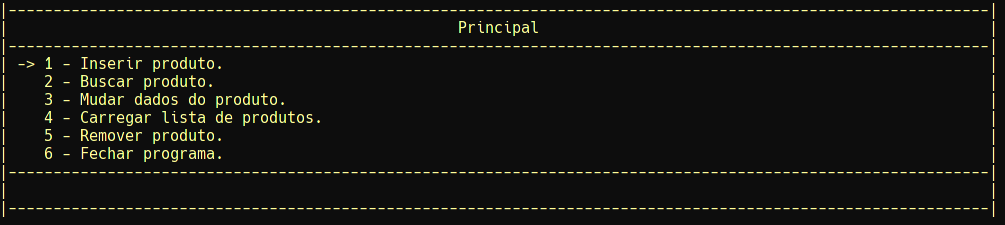
\includegraphics[width=\textwidth]{principal.png}
    \caption{\label{fig:pricipal}Menu principal}
\end{figure}

\begin{figure}[!htb]
    \centering
    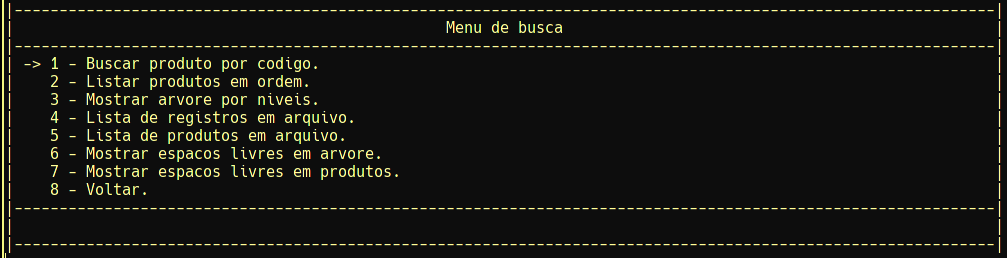
\includegraphics[width=\textwidth]{buscar}
    \caption{\label{fig:buscar}Menu de busca}
\end{figure}

\begin{figure}[!htb]
    \centering
    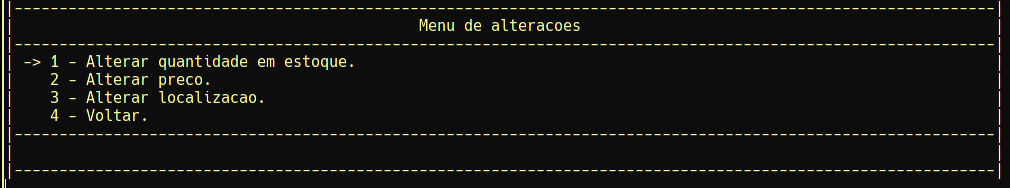
\includegraphics[width=\textwidth]{mudar}
    \caption{\label{fig:mudar}Menu de alterar}
\end{figure}

\begin{figure}[!htb]
    \centering
    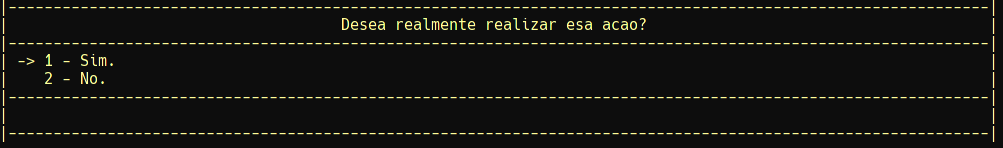
\includegraphics[width=\textwidth]{confirmar}
    \caption{\label{fig:confirmar}Menu de confirmar}
\end{figure}

\cleardoublepage
\section{Estruturas de Dados}\label{Estruturas de Dados}

Segue abaixo as principais estruturas de dados utilizadas ao longo da execução do programa.

\subsection{Estrutura do Menu}\label{Estrutura do Menu}

Estruturas encarregadas de definir o menu.

\begin{lstlisting}
typedef int CallbackFunct(ArgStack head);
typedef void HeaderFunct();
typedef void FooterFunct();

typedef struct entryNode {
    int number;
	char entryMessage[MESSAGE_SIZE];
    CallbackFunct *funct;
    struct entryNode *next;
    struct entryNode *prev;
}Entry;

typedef Entry* EntryList;

typedef struct {
    FooterFunct *footer;
    HeaderFunct *header;
    EntryList first;
    EntryList selected;
}Menu;
\end{lstlisting}

\cleardoublepage
\subsection{Estruturas do arquivo de índices}\label{Estruturas do arquivo de índices}

Dados gravados no arquivo ``index.bin'' para representar a árvore B.

\begin{lstlisting}
typedef struct {
    int regRoot;
    int regLast;
    int regFree;
}IndexHead;

typedef struct {
    int key;
    int position;
    int leftChild;
    int rightChild;
}RegistryField;

typedef struct {
    int numberOfKeys;
	int key[ORDER];
	int position[ORDER];
	int children[ORDER + 1];
}Registry;
\end{lstlisting}

\cleardoublepage
\subsection{Estruturas do arquivo de Dados}\label{Estruturas do arquivo de Dados}

Dados gravados no arquivo ``data.bin'' para representar os dados dos produtos contidos na árvore B.

\begin{lstlisting}

#define MAX_NAME 51

#define MAX_LOCAL 101

typedef struct {
    int regLast;
    int regFree;
}DataHead;

typedef struct {
    int code;
    char name[MAX_NAME];
    int number;
    float value;
    char local[MAX_LOCAL];
}Product;

\end{lstlisting}

\end{document}
